\documentclass[12pt,a4paper]{article}
\usepackage{graphicx}

\title{Praktikum Physik - Tr\"agheitsmoment}
\author{Simon Marti, Patricia Schwab, Mirco Kocher}
\date{02.03.2012}

\begin{document}
\maketitle

%%
% Ziel
%%
\section*{Ziel}
 Berechnung der Tr\"agheitsmomente unterschiedlicher K\"orper durch Messung der Schwingungsperiode und Verifizierung des Satzes von Steiner.

%%
% Motivation
%%
\section*{Motivation}
Der Versuch des Tr\"agheitsmoments eignet sich gut als Einstieg ins Physikpraktikum. Ausserdem kann mit den gemessenen Daten eine umfassende Fehlerrechnung durchgef\"uhrt werden.

%%
% Theorie
%%
\section*{Theorie}

Tr\"agheitsmoment
\[  J = \sum mr^2\ \]
\[  J_{zylinder} = \frac{m}{12}(h^2 + 3R^2) \]
\[ J_{quader} = \frac{m}{12}(l^2 + b^2) \]
Rotationsenergie
\[ E_{rot} = \frac{1}{2}J\omega^2 \]
Drehimpuls
\[ L = J\omega \]
Schwingung
\[ J = \frac{T^2k}{4\pi^2} \]

%%
% Experiment
%%
\section*{Experiment}

% Aufbau und Ablauf
\subsection*{Aufbau und Ablauf}
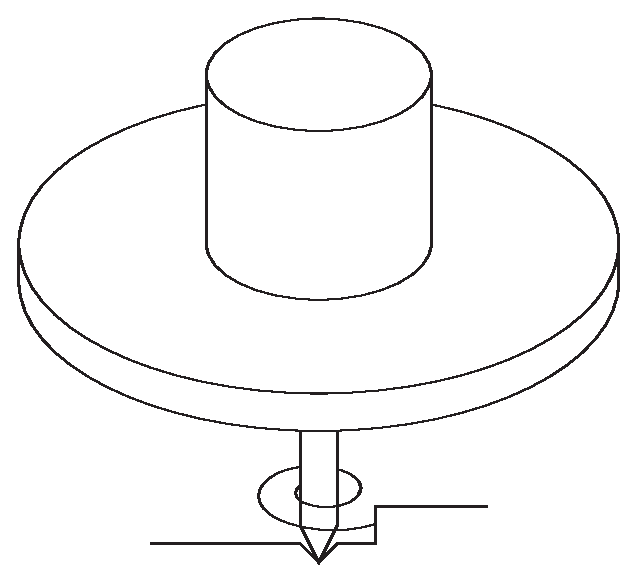
\includegraphics[width=6cm]{illustration11.pdf}

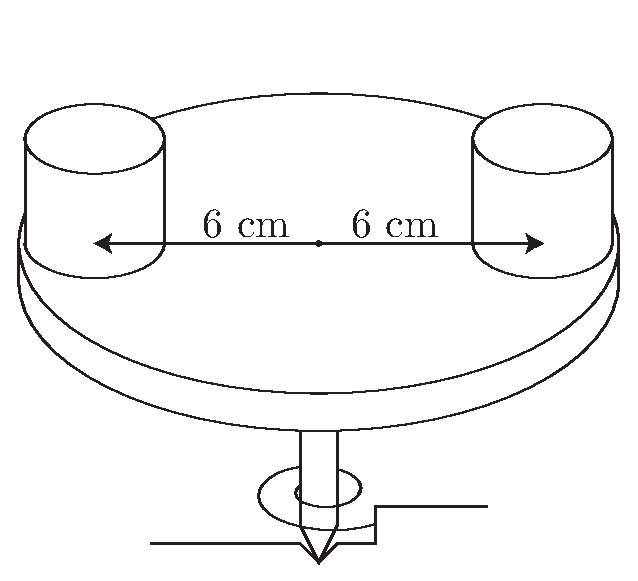
\includegraphics[width=6cm]{illustration12.pdf}

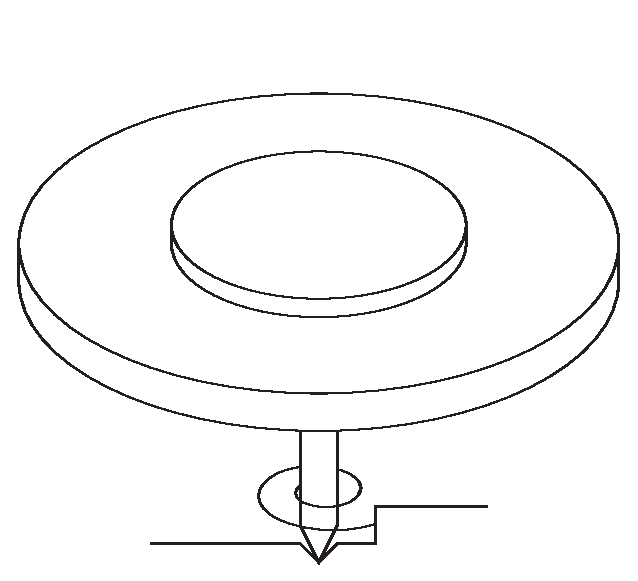
\includegraphics[width=6cm]{illustration21.pdf}

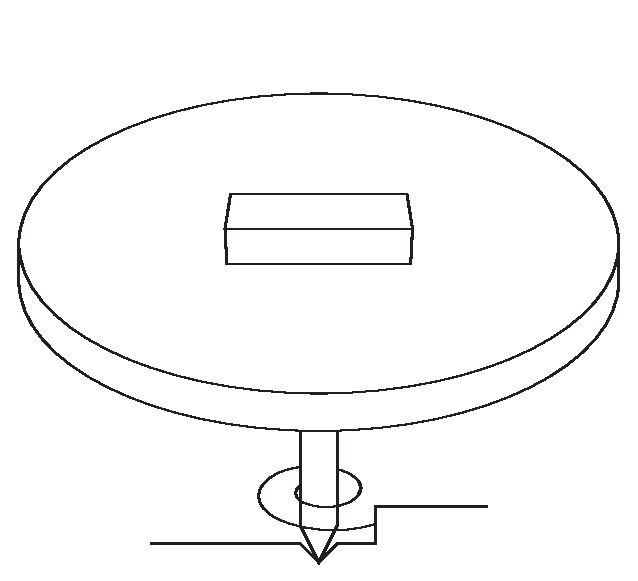
\includegraphics[width=6cm]{illustration22.pdf}

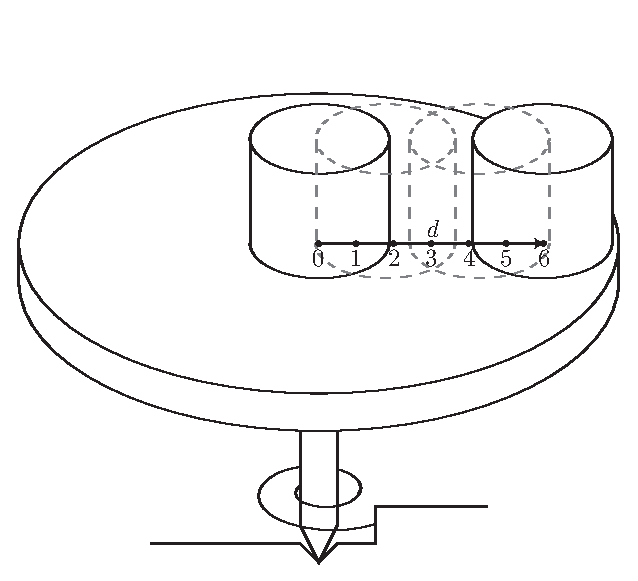
\includegraphics[width=10cm]{illustration3.pdf}

% Rohdaten
\subsection*{Rohdaten}

\begin{tabular}{|l|r|r|r|r|r|r|}
\hline
$d$&$T_1$&$T_2$&$T_3$&$T_4$&$T_5$&avg \\
\hline
0&12.4&12.3&12.4&12.65&12.45&12.44\\
1&12.55&12.7&12.75&12.7&12.55&12.65\\
2&12.4&13.55&13.25&13.4&13.25&13.17\\
3&14.5&14.5&14.4&14.5&14.5&14.48\\
4&16&15.8&15.8&16&16.05&15.93\\
5&17.6&17.55&17.7&17.65&17.5&17.6\\
6&19.35&19.5&19.7&19.45&19.45&19.49\\
\hline
\end{tabular}

\begin{tabular}{|l|l|l|l|l|}
\hline
$T_{1}$&$T_{2}$&$T_{3}$&$T_{4}$&$T_{5}$\\
\hline
14.95 s&15.1 s&14.6 s&15.0 s&15.15 s\\
\hline
\hline
$T_{6}$&$T_{7}$&$T_{8}$&$T_{9}$&$T_{10}$\\
\hline
15.05 s&15.1 s&15.1 s&15.0 s&15.0 s\\
\hline
\end{tabular}

% Kontrollrechnung
\subsection*{Kontrollrechnung}

% Auswertung
\subsection*{Auswertung}

%%
% Diskussion
%%
\section*{Diskussion}

\end{document}